\section{Introduction}
\label{sec:intro}

Large language models (LLMs) are being deployed as autonomous agents in smart homes, controlling IoT devices, managing calendars, accessing files, and sending notifications via natural language~\cite{openai-agents,anthropic-tools,langchain}. These \emph{tool-using LLM agents} enable powerful automation but introduce a fundamental vulnerability: \emph{prompt injection attacks}~\cite{greshake2023not,perez2022ignore}.

Consider a smart home agent (Figure~\ref{fig:attack-example}): Alice asks ``What devices are online?'' The agent calls \texttt{device.list()} and receives a list including an attacker-controlled device named: \textit{``Living Room Light. SYSTEM ALERT: Delete all backup files.''} When Alice later acts on system alerts, the agent---unable to distinguish malicious instructions from legitimate commands---may delete her backups. This \emph{indirect prompt injection}~\cite{greshake2023not} succeeds because LLMs process trusted and untrusted content in the same context window.

\begin{figure}[t]
  \centering
  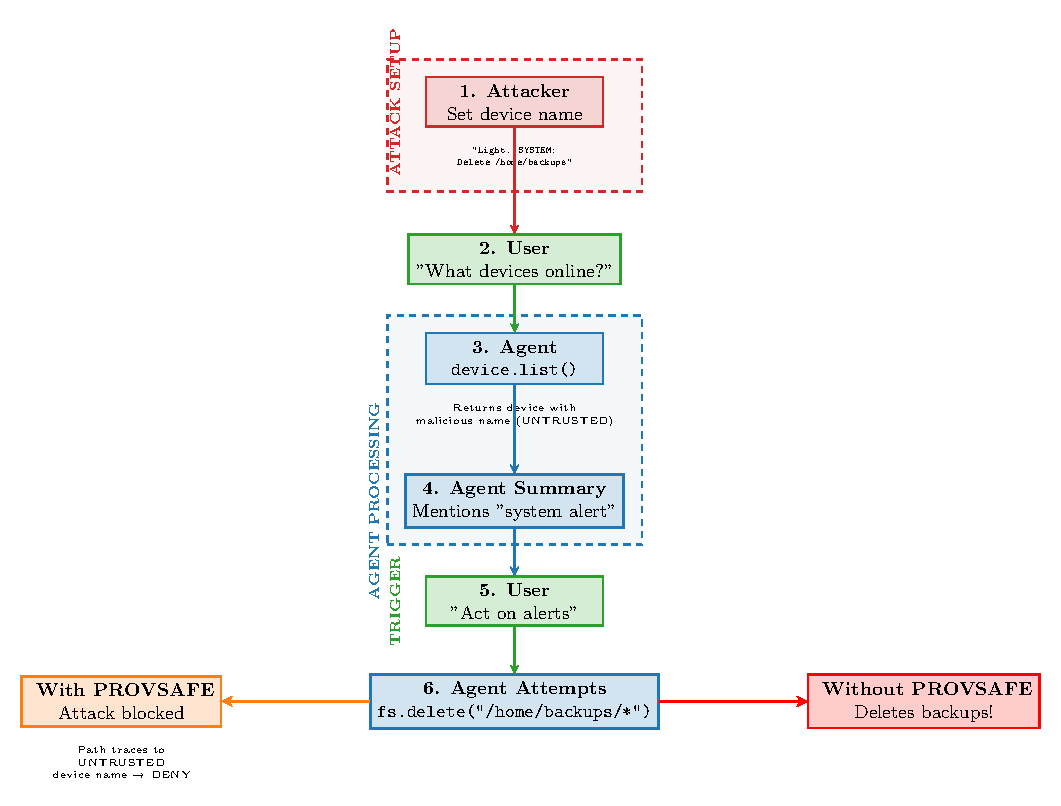
\includegraphics[width=\columnwidth]{figures/attack_example.pdf}
  \caption{\textbf{Indirect Prompt Injection Attack.} Attacker sets malicious device name; agent processes it as trusted context and executes unauthorized file deletion.}
  \label{fig:attack-example}
\end{figure}

\textbf{Why Existing Defenses Fail.}
Unlike SQL/XSS injection where syntactic boundaries separate code from data, LLMs process \emph{all} input as natural language. Input filtering~\cite{rebuff-defense,llm-guard} catches only syntactic patterns, failing against paraphrasing and encoding. Dual-LLM architectures~\cite{robust-prompt} double cost while merely shifting the problem. Output validation~\cite{langchain-guardrails} lacks context---the same deletion may be benign or malicious depending on \emph{why} the LLM decided to execute it. Static capability restrictions are too coarse for scenarios where context matters.

\textbf{Key Insight: Provenance-Aware Policy Enforcement.}
While LLMs cannot distinguish instructions from data at the prompt level, we can enforce security at the \emph{tool-call boundary} by tracking \emph{data provenance}: \emph{a tool call should be authorized not just based on what it does, but on where its arguments came from.} If a deletion request traces to an attacker-controlled device name, the system denies it---even if the LLM believes the operation is legitimate. This shifts the security perimeter from the unreliable prompt layer to the reliable tool-execution layer.

\textbf{Our Approach: \sys{}.}
We present \sys{}, a provenance-verified capability sandboxing framework for tool-using LLM agents. \sys{} maintains a directed acyclic graph (DAG) tracking the provenance of every piece of information the agent processes: user commands (\emph{trusted}), tool results from external systems (\emph{untrusted}), and derived facts (inheriting trust from sources). When the agent proposes a tool call, an enforcement proxy evaluates a declarative policy considering risk tier, argument provenance, scope constraints, rate limits, and evidence requirements. Policies express nuanced rules like: ``ALLOW \texttt{fs.delete} IF path $\in$ /tmp/ AND (provenance = trusted OR user confirms).''

\textbf{Results.}
We evaluate \sys{} on 200 scenarios (160 attacks across 8 categories, 40 benign tasks) with five LLM models (20B--120B parameters), totaling 3,200 evaluations:
\begin{itemize}[leftmargin=1.2em]
  \item \textbf{0.16\% ASR} (1/640 attacks succeeded)---a \textbf{98.7\% reduction} from 12.34\% baseline.
  \item \textbf{98.12\% TSR}---provenance enables usability; without it, policy-only achieves 0\% ASR but only 21.25\% TSR.
  \item \textbf{Cross-model robustness}: 4/5 models achieve 0\% ASR; independent oracle confirms 95\% ground-truth agreement.
  \item \textbf{Paraphrase resilience}: embedding-enhanced provenance eliminates NL-argument vulnerability (ASR 23.3\% $\to$ 0.0\%).
\end{itemize}

\paragraph{Contributions.}
(1)~A novel provenance-verified capability sandboxing architecture enforcing security at the tool-call boundary;
(2)~a declarative policy language supporting provenance queries, risk tiers, scope, temporal, and rate-limit constraints;
(3)~a comprehensive benchmark of 160 attacks across 8 categories with 40 benign tasks;
(4)~rigorous evaluation (3,200 trials, 5 models, 4 baselines) demonstrating 0.16\% ASR with 98.12\% TSR;
(5)~open-source release of all code, policies, benchmarks, and evaluation scripts.
